% Created 2017-04-11 Tue 15:34
% Intended LaTeX compiler: pdflatex
\documentclass[presentation]{beamer}
\usepackage[utf8]{inputenc}
\usepackage[T1]{fontenc}
\usepackage{graphicx}
\usepackage{grffile}
\usepackage{longtable}
\usepackage{wrapfig}
\usepackage{rotating}
\usepackage[normalem]{ulem}
\usepackage{amsmath}
\usepackage{textcomp}
\usepackage{amssymb}
\usepackage{capt-of}
\usepackage{hyperref}
\usetheme{default}
\author{Petr Blaho}
\date{\today}
\title{PA200 - OpenStack - Technical Insight}
\hypersetup{
 pdfauthor={Petr Blaho},
 pdftitle={PA200 - OpenStack - Technical Insight},
 pdfkeywords={},
 pdfsubject={},
 pdfcreator={Emacs 25.1.1 (Org mode 9.0.5)}, 
 pdflang={English}}
\begin{document}

\maketitle

\begin{frame}[label={sec:org7580345}]{OpenStack Overview}
\begin{block}{Schema}
\begin{center}
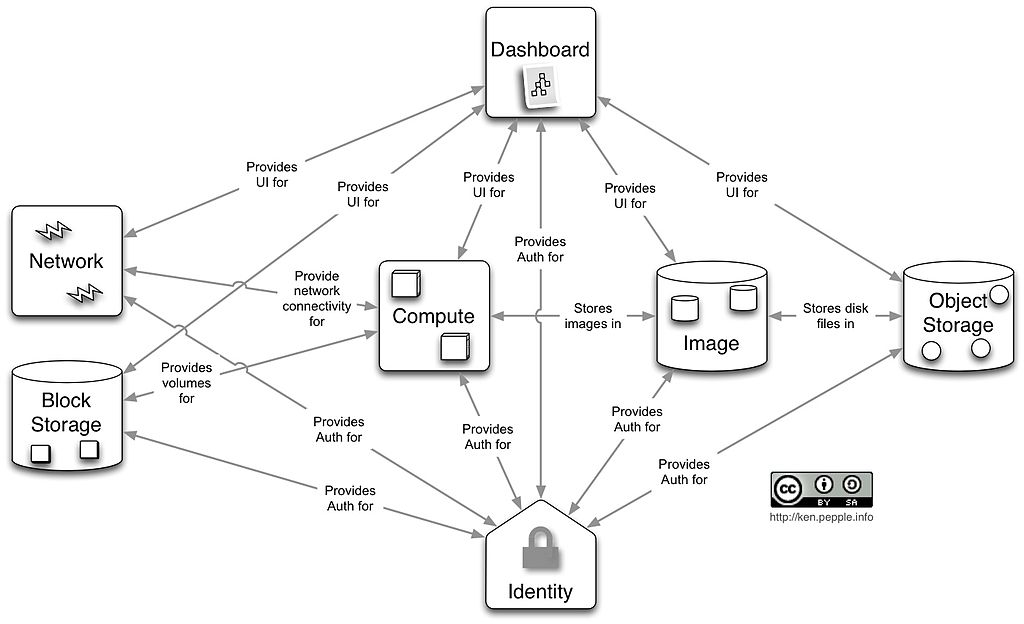
\includegraphics[width=.9\linewidth]{./openstack.jpg}
\end{center}
\end{block}
\begin{block}{Conceptual Schema}
\begin{center}
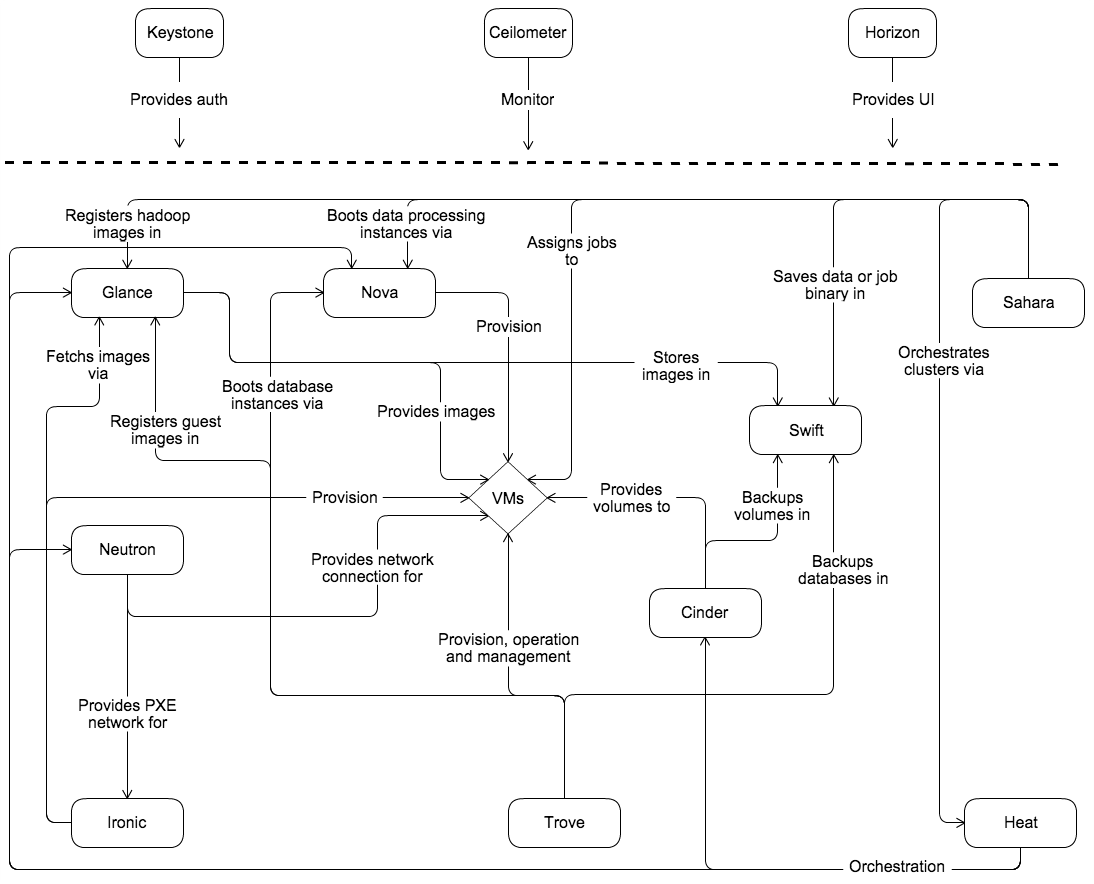
\includegraphics[width=.9\linewidth]{./openstack-conceptual-arch-kilo.png}
\end{center}
\end{block}
\begin{block}{Logical Schema}
\begin{center}
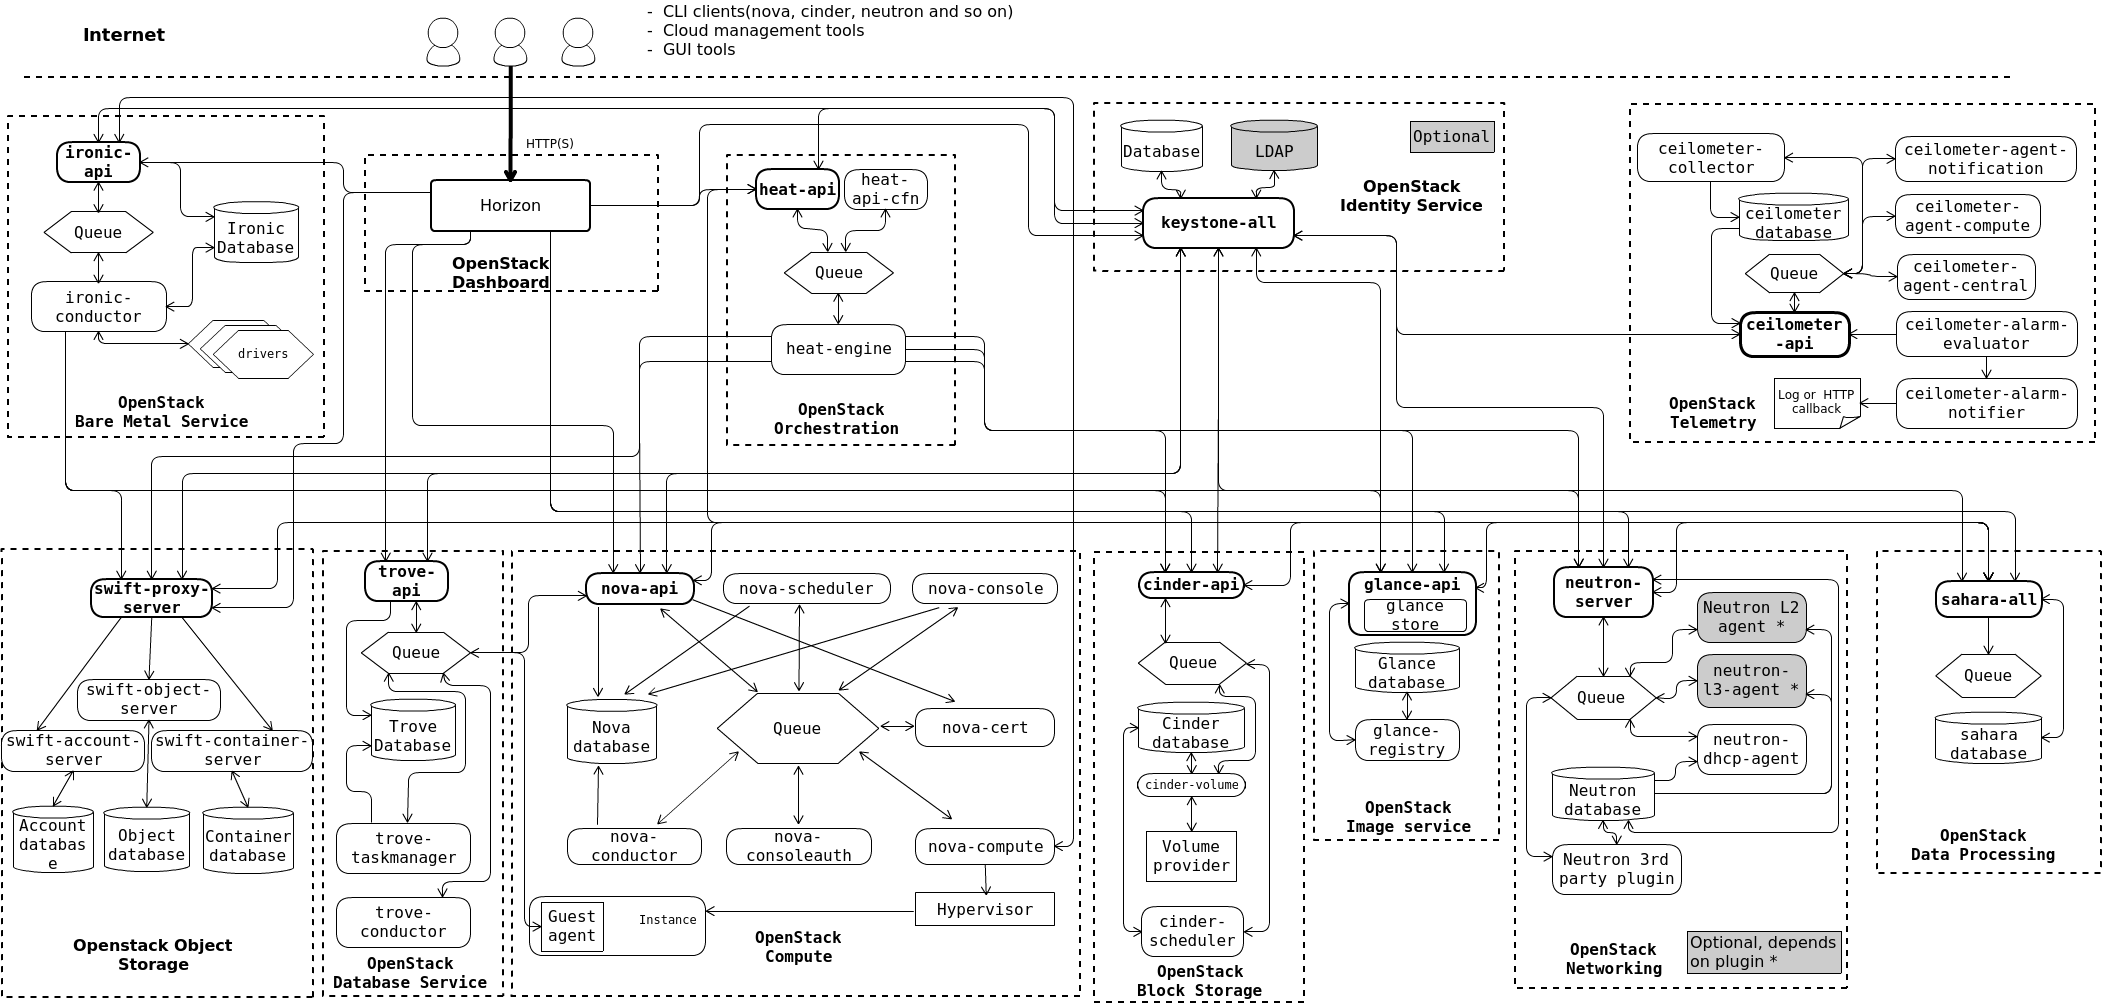
\includegraphics[width=.9\linewidth]{./openstack-logical-arch-kilo.png}
\end{center}
\end{block}
\end{frame}
\begin{frame}[fragile,label={sec:orgdf62090}]{OpenStack Components (Projects)}
 \begin{block}{Identity (Keystone)}
\begin{itemize}
\item manages users, projects, domains, roles, groups
\item authorization scopes - unscoped, project, domain
\item role-based access control (RBAC)
\end{itemize}
\begin{verbatim}
"identity:create_user": "role:admin and domain_id:%(user.domain_id)s"
\end{verbatim}
\end{block}
\begin{block}{Dashboard (Horizon)}
\begin{itemize}
\item web UI
\item allow to manage:
\item users, groups, roles, projects
\item instances, images, volumes
\item quotas, cloud resources, \ldots{}
\end{itemize}
\end{block}
\begin{block}{Compute (Nova)}
\begin{block}{Hypervisors}
\begin{itemize}
\item Baremetal
\item Docker
\item Hyper-V
\item Kernel-based Virtual Machine (KVM)
\item Linux Containers (LXC)
\item Quick Emulator (QEMU)
\item User Mode Linux (UML)
\item VMware vSphere
\item Xen
\item Feature matrix - \url{https://docs.openstack.org/developer/nova/support-matrix.html}
\end{itemize}
\end{block}
\begin{block}{Services}
\begin{itemize}
\item nova-api service - API endpoints
\item nova-api-metadata service - metadata about instances
\item nova-compute service - talks with hypervisors via XenAPI, libvirt, VMWareAPI
\item nova-placement-api service - tracks resource provider inventories and usages
\item nova-scheduler service - decides on which compute host will instance be run
\item nova-conductor module - mediator between nova-compute and database
\end{itemize}
\end{block}
\begin{block}{Services cont.}
\begin{itemize}
\item nova-consoleauth daemon - authorizes tokens for console proxies users
\item nova-novncproxy, nova-spicehtml5proxy, nova-xvpvncproxy daemons
\end{itemize}
\end{block}
\begin{block}{Queue}
\begin{itemize}
\item central hub for messaging
\item RabbitMQ
\item ZeroMQ
\item another AMQP
\end{itemize}
\end{block}
\begin{block}{SQL database}
\begin{itemize}
\item store build-time and run-time states, like:
\item available instance types
\item instances in use
\item available networks
\item projects
\item any DB supported by SQLAlchemy
\item SQLite3, MySQL, MariaDB, PostgreSQL
\end{itemize}
\end{block}
\end{block}
\begin{block}{Object Storage (Swift)}
\begin{block}{Characteristics}
\begin{itemize}
\item objects have URL
\item objects are 3x replicated over zones (group of drives, node, rack)
\item objects have metadata
\item RESTful HTTP API
\item objects can be anywhere in the cluster
\item cluster scales in a linear way by adding nodes without downtime
\end{itemize}
\end{block}
\begin{block}{Components}
\begin{itemize}
\item proxy servers - handle incoming API requests
\item rings - map logical names of data to locations on particular disks
\item zones - isolate data from other zones
\item account and containers - Account -> Containers -> Objects
\item objects - data
\item partitions - stores objects, account and container dbs, help manage locations where data lives
\end{itemize}
\end{block}
\begin{block}{Schema}
\begin{center}
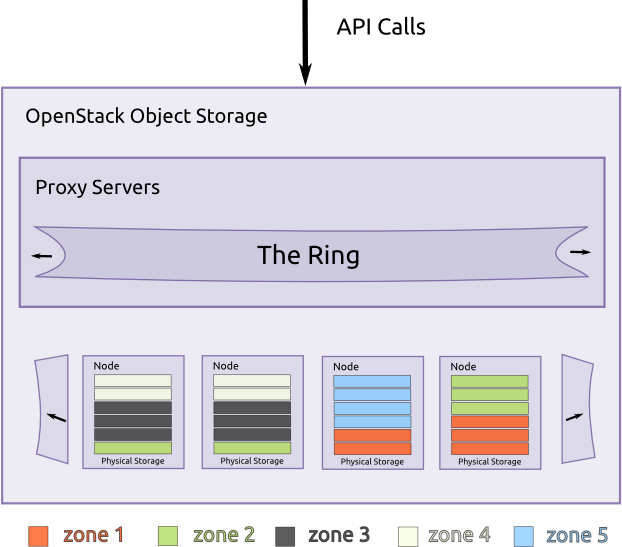
\includegraphics[width=.9\linewidth]{./objectstorage-buildingblocks.png}
\end{center}
\end{block}
\end{block}
\begin{block}{Block Storage (Cinder)}
\begin{block}{Backends}
\begin{itemize}
\item default implementation uses LVM
\item NFS
\item GlusterFS
\item others
\end{itemize}
\end{block}
\begin{block}{Features}
\begin{itemize}
\item volumes and snapshots management
\item migrating volumes
\item bandwidth limiting for volume copying
\item oversubscription
\item expose backend specific capabilities
\end{itemize}
\end{block}
\end{block}
\begin{block}{Networking (Neutron)}
\begin{block}{Features}
\begin{itemize}
\item Layer 2 - networks, ports, segments
\item Layer 3 - floating IPs, routers, subnets
\item Services - LBaaS, FWaaS, VPNaaS
\end{itemize}
\end{block}
\begin{block}{Architecture}
\begin{itemize}
\item neutron-*-agent - run on each hypervisor
\item neutron-dhcp-agent - DHCP
\item neutron-l3-agent - L3/NAT forwarding to provide external network access to VMs
\item neutron-metering-agent - L3 traffic metering
\end{itemize}
\end{block}
\end{block}
\begin{block}{Image Service (Glance)}
\begin{itemize}
\item stores disk and server images for instances to boot from
\item can use Cinder as backend
\end{itemize}
\end{block}
\begin{block}{Telemetry (Ceilometer)}
\begin{block}{Features}
\begin{itemize}
\item aodh - alarms
\item gnocchi - measurements - \url{https://docs.openstack.org/admin-guide/telemetry-measurements.html}
\item panko - events
\item data retrieval - query language to get data and statistics
\item data pipelines - processes data before published
\end{itemize}
\end{block}
\begin{block}{Architecture}
\begin{itemize}
\item backends:
\item measurements - gnocchi
\item alarms - MySQL, PostgreSQL
\item events - ElasticSearch, MongoDB, MySQL, PostgreSQL, HBase
\item hypervisors: libvirt, Hyper-V, XEN, VMWare vSphere
\item networking: OpenStack, SDN - OpenDaylight, OpenContrail
\end{itemize}
\end{block}
\end{block}
\begin{block}{Orchestration (Heat)}
\begin{itemize}
\item orchestrating clouds
\item automatically configures resources
\item deploys resources
\end{itemize}
\end{block}
\begin{block}{Bare-Metal Provisioning (Ironic)}
\begin{itemize}
\item provides bare metal machines instead of VM
\item uses PXE and agent to deploy
\end{itemize}
\end{block}
\begin{block}{Database (Trove)}
\begin{itemize}
\item MySQL, MongoDB, Cassandra
\end{itemize}
\end{block}
\begin{block}{other}
\begin{itemize}
\item Elastic Map Reduce (Sahara)
\item Messaging Service (Zaqar)
\item Shared Filesystems (Manila)
\item DNS Service (Designate)
\item Key Management (Barbican)
\item Containers (Magnum)
\item Application Catalog (Murano)
\item Governance (Congress)
\end{itemize}
\end{block}
\end{frame}
\begin{frame}[label={sec:org0e76afc}]{OpenStack Clients (CLI, python, web UI)}
\begin{itemize}
\item demo
\end{itemize}
\end{frame}
\begin{frame}[label={sec:orgaf38fdf}]{OpenStack Contribution}
\begin{itemize}
\item \url{https://www.openstack.org/}
\item \url{https://review.openstack.org/}
\end{itemize}
\end{frame}
\end{document}
